\chapter{Slika}
We can se one cute cat on the image below.
\begin{figure}[ht!]
  \centering
  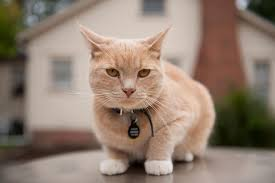
\includegraphics{images/cat.jpg}
  \caption{Cute cat}
  \label{fig:cute_cat}
\end{figure}

Figure \ref{fig:cute_cat} shows one cute cat.

\begin{figure}[ht!]
  \centering
  \begin{subfigure}[b]{0.4\linewidth}
    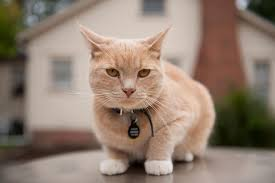
\includegraphics[width=\linewidth]{images/cat.jpg}
    \caption{Left cat.}
  \end{subfigure}
  \begin{subfigure}[b]{0.4\linewidth}
    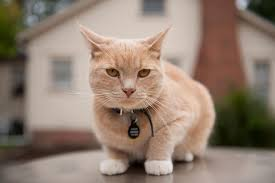
\includegraphics[width=\linewidth]{images/cat.jpg}
    \caption{Right cat.}
  \end{subfigure}
  \caption{The same cute cat. Two times.}
  \label{fig:two_cats}
\end{figure}


\begin{figure}[ht!]

  \centering
  \begin{subfigure}[b]{0.2\linewidth}
    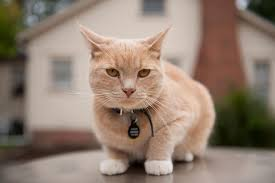
\includegraphics[width=\linewidth]{images/cat.jpg}
     \caption{Left cat.}
  \end{subfigure}
  \begin{subfigure}[b]{0.2\linewidth}
    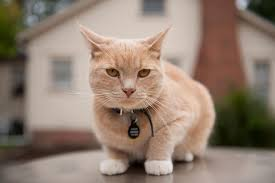
\includegraphics[width=\linewidth]{images/cat.jpg}
    \caption{Middle cat.}
  \end{subfigure}
  \begin{subfigure}[b]{0.2\linewidth}
    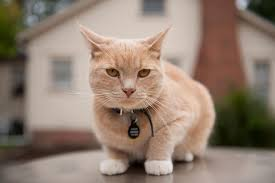
\includegraphics[width=\linewidth]{images/cat.jpg}
    \caption{Right cat.}
  \end{subfigure}

  \begin{subfigure}[b]{0.5\linewidth}
    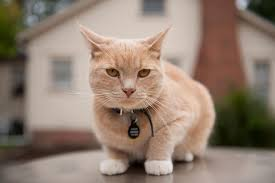
\includegraphics[width=\linewidth]{images/cat.jpg}
    \caption{Big cat.}
  \end{subfigure}

  \caption{The same cute cat. Multiple times.}
  \label{fig:multiple_cats}
\end{figure}